% TEMPLATE.TEX
%
% Time-stamp: <2013-03-26 11:09 olenz>
%
% This is an extensively documented LaTeX file that shows how to
% produce a good-looking document with current LaTeX (11/2012).
%
% IMPORTANT!
%
%   Some obsolete commands and packages
% ----------|-------------------------------
% obsolete  |     Replacement in LATEX 2ε
% ----------|-------------------------------
%           | local            global/switch
% ----------|-------------------------------
% {\bf ...} | \textbf{...}     \bfseries
%     -     | \emph{...}       \em
% {\it ...} | \textit{...}     \itshape
%     -     | \textmd{...}     \mdseries
% {\rm ...} | \textrm{...}     \rmfamily
% {\sc ...} | \textsc{...}     \scshape
% {\sf ...} | \textsf{...}     \sffamily
% {\sl ...} | \textsl{...}     \slshape
% {\tt ...} | \texttt{...}     \ttfamily
%     -     | \textup{...}     \upshape
%
% DON'T USE \\ TO MAKE LINEBREAKS, INSTEAD JUST LEAVE A BLANK LINE!
%
\RequirePackage[l2tabu,orthodox]{nag} % turn on warnings because of bad style
\documentclass[a4paper,11pt,bibtotoc]{scrartcl}
%
%%%%%%%%%%%%%%%%%%%%%%%%%%%%%%%%%%%%
% KOMA CLASSES
%%%%%%%%%%%%%%%%%%%%%%%%%%%%%%%%%%%%
%
% The class "scrartcl" is one of the so-called KOMA-classes, a set of
% very well done LaTeX-classes that produce a very European layout
% (e.g. titles with a sans-serif font).
% 
% The KOMA classes have extensive documentation that you can access
% via the commands:
%   texdoc scrguide # in German
%   texdoc scrguien # in English
%   
%
% The available classes are:
%
% scrartcl - for "articles", typically for up to ~20 pages, the
%            highest level sectioning command is \section
%
% scrreprt - for "reports", typically for up to ~200 pages, the
%            highest level sectioning command is \chapter
%
% scrbook  - for "books", for more than 200 pages, the highest level
%            sectioning command is \part.
%
% USEFUL OPTIONS
%
% a4paper  - Use a4 paper instead of the default american letter
%            format.
%
% 11pt, 12pt, 10pt 
%          - Use a font with the given size.
%
% bibtotoc - Add the bibliography to the table of contents
%
% The KOMA-script classes have plenty of options to modify

% This allows to type UTF-8 characters like ä,ö,ü,ß
\usepackage[utf8]{inputenc}

% Default fixed font does not support bold face
\DeclareFixedFont{\ttb}{T1}{txtt}{bx}{n}{12} % for bold
\DeclareFixedFont{\ttm}{T1}{txtt}{m}{n}{12}  % for normal

% Custom colors
\usepackage{color}
\definecolor{deepblue}{rgb}{0,0,0.5}
\definecolor{deepred}{rgb}{0.6,0,0}
\definecolor{deepgreen}{rgb}{0,0.5,0}

\usepackage[T1]{fontenc}        % Tries to use Postscript Type 1 Fonts for better rendering
\usepackage{lmodern}            % Provides the Latin Modern Font which offers more glyphs than the default Computer Modern
\usepackage[intlimits]{amsmath} % Provides all mathematical commands

\usepackage{hyperref}           % Provides clickable links in the PDF-document for \ref
\usepackage{grffile}            % Allow you to include images (like graphicx). Usage: \includegraphics{path/to/file}

% Allows to set units
\usepackage[ugly]{units}        % Allows you to type units with correct spacing and font style. Usage: $\unit[100]{m}$ or $\unitfrac[100]{m}{s}$

% Additional packages
\usepackage{url}                % Lets you typeset urls. Usage: \url{http://...}
\usepackage{breakurl}           % Enables linebreaks for urls
\usepackage{xspace}             % Use \xpsace in macros to automatically insert space based on context. Usage: \newcommand{\es}{ESPResSo\xspace}
\usepackage{xcolor}             % Obviously colors. Usage: \color{red} Red text
\usepackage{booktabs}           % Nice rules for tables. Usage \begin{tabular}\toprule ... \midrule ... \bottomrule

% Source code listings
\usepackage{listings}           % Source Code Listings. Usage: \begin{lstlisting}...\end{lstlisting}
\lstloadlanguages{python}       % Default highlighting set to "python"

% Allow for bold math fonts
\usepackage{bm}


\usepackage{graphicx} % Required for including images                                                                 
% Python style for highlighting
\newcommand\pythonstyle{\lstset{
language=Python,
basicstyle=\ttm,
otherkeywords={self},             % Add keywords here
keywordstyle=\ttb\color{deepblue},
emph={MyClass,__init__},          % Custom highlighting
emphstyle=\ttb\color{deepred},    % Custom highlighting style
stringstyle=\color{deepgreen},
frame=tb,                         % Any extra options here
showstringspaces=false            % 
}}


% Python environment
\lstnewenvironment{python}[1][]
{
\pythonstyle
\lstset{#1}
}
{}                                                                 
                                                                 
\begin{document}

\titlehead{Simulation Methods in Physics I \hfill WS 2017/2018}
\title{Worksheet 1: Integrators}
\author{Cameron N. Stewart}
\date{\today}
\publishers{Institute for Computational Physics, University of
  Stuttgart}
\maketitle

\tableofcontents

\section{Introduction}

In this worksheet we use will be using molecular dynamics simulation
to look at the trajectory of a cannonball under the influence of
gravity, friction, and wind and at a 2D representation of the solar
system. We will be studying the behavior of a few different
integrators in the latter simulation.

\section{Cannonball}
\subsection{Simulating a cannonball}
In this first exercise we simulate a cannonball in 2D under gravity in
the absence of friction. The cannonball has a mass
$m = \unit[2.0]{kg}$ ,we take gravitational acceleration to be
$g = \unitfrac[9.81]{m}{s^2}$, the cannonball has initial position
$\bm{x}(0) = \bm{0}$, and initial velocity
$\bm{v}(0) = \begin{pmatrix} 50 \\ 50\\ \end{pmatrix}
\unitfrac{m}{s}$. We will use the simple Euler scheme to integrate or
system. This is given by:
\begin{align}
  \bm{x}(t+\Delta t) &= \bm{x}(t) + \bm{v}(t) \Delta t \\
  \bm{v}(t+\Delta t) &= \bm{v}(t) + \frac{\bm{F}(t)}{m} \Delta t 
\end{align}                       
This is essentially just the Taylor expansion of position and velocity
cut off below second order. We implement the simple Euler algorithm in
python as follows:
\begin{python}
def step_euler(x, v, dt):
    f = compute_forces(x)
    x += v*dt
    v += f*dt/m    
    return x, v
\end{python}
The forces are computed simply with

\begin{python}
def compute_forces(x):
    f = np.array([0.0, -m*g])
    return f
\end{python}

\begin{figure}[t]
  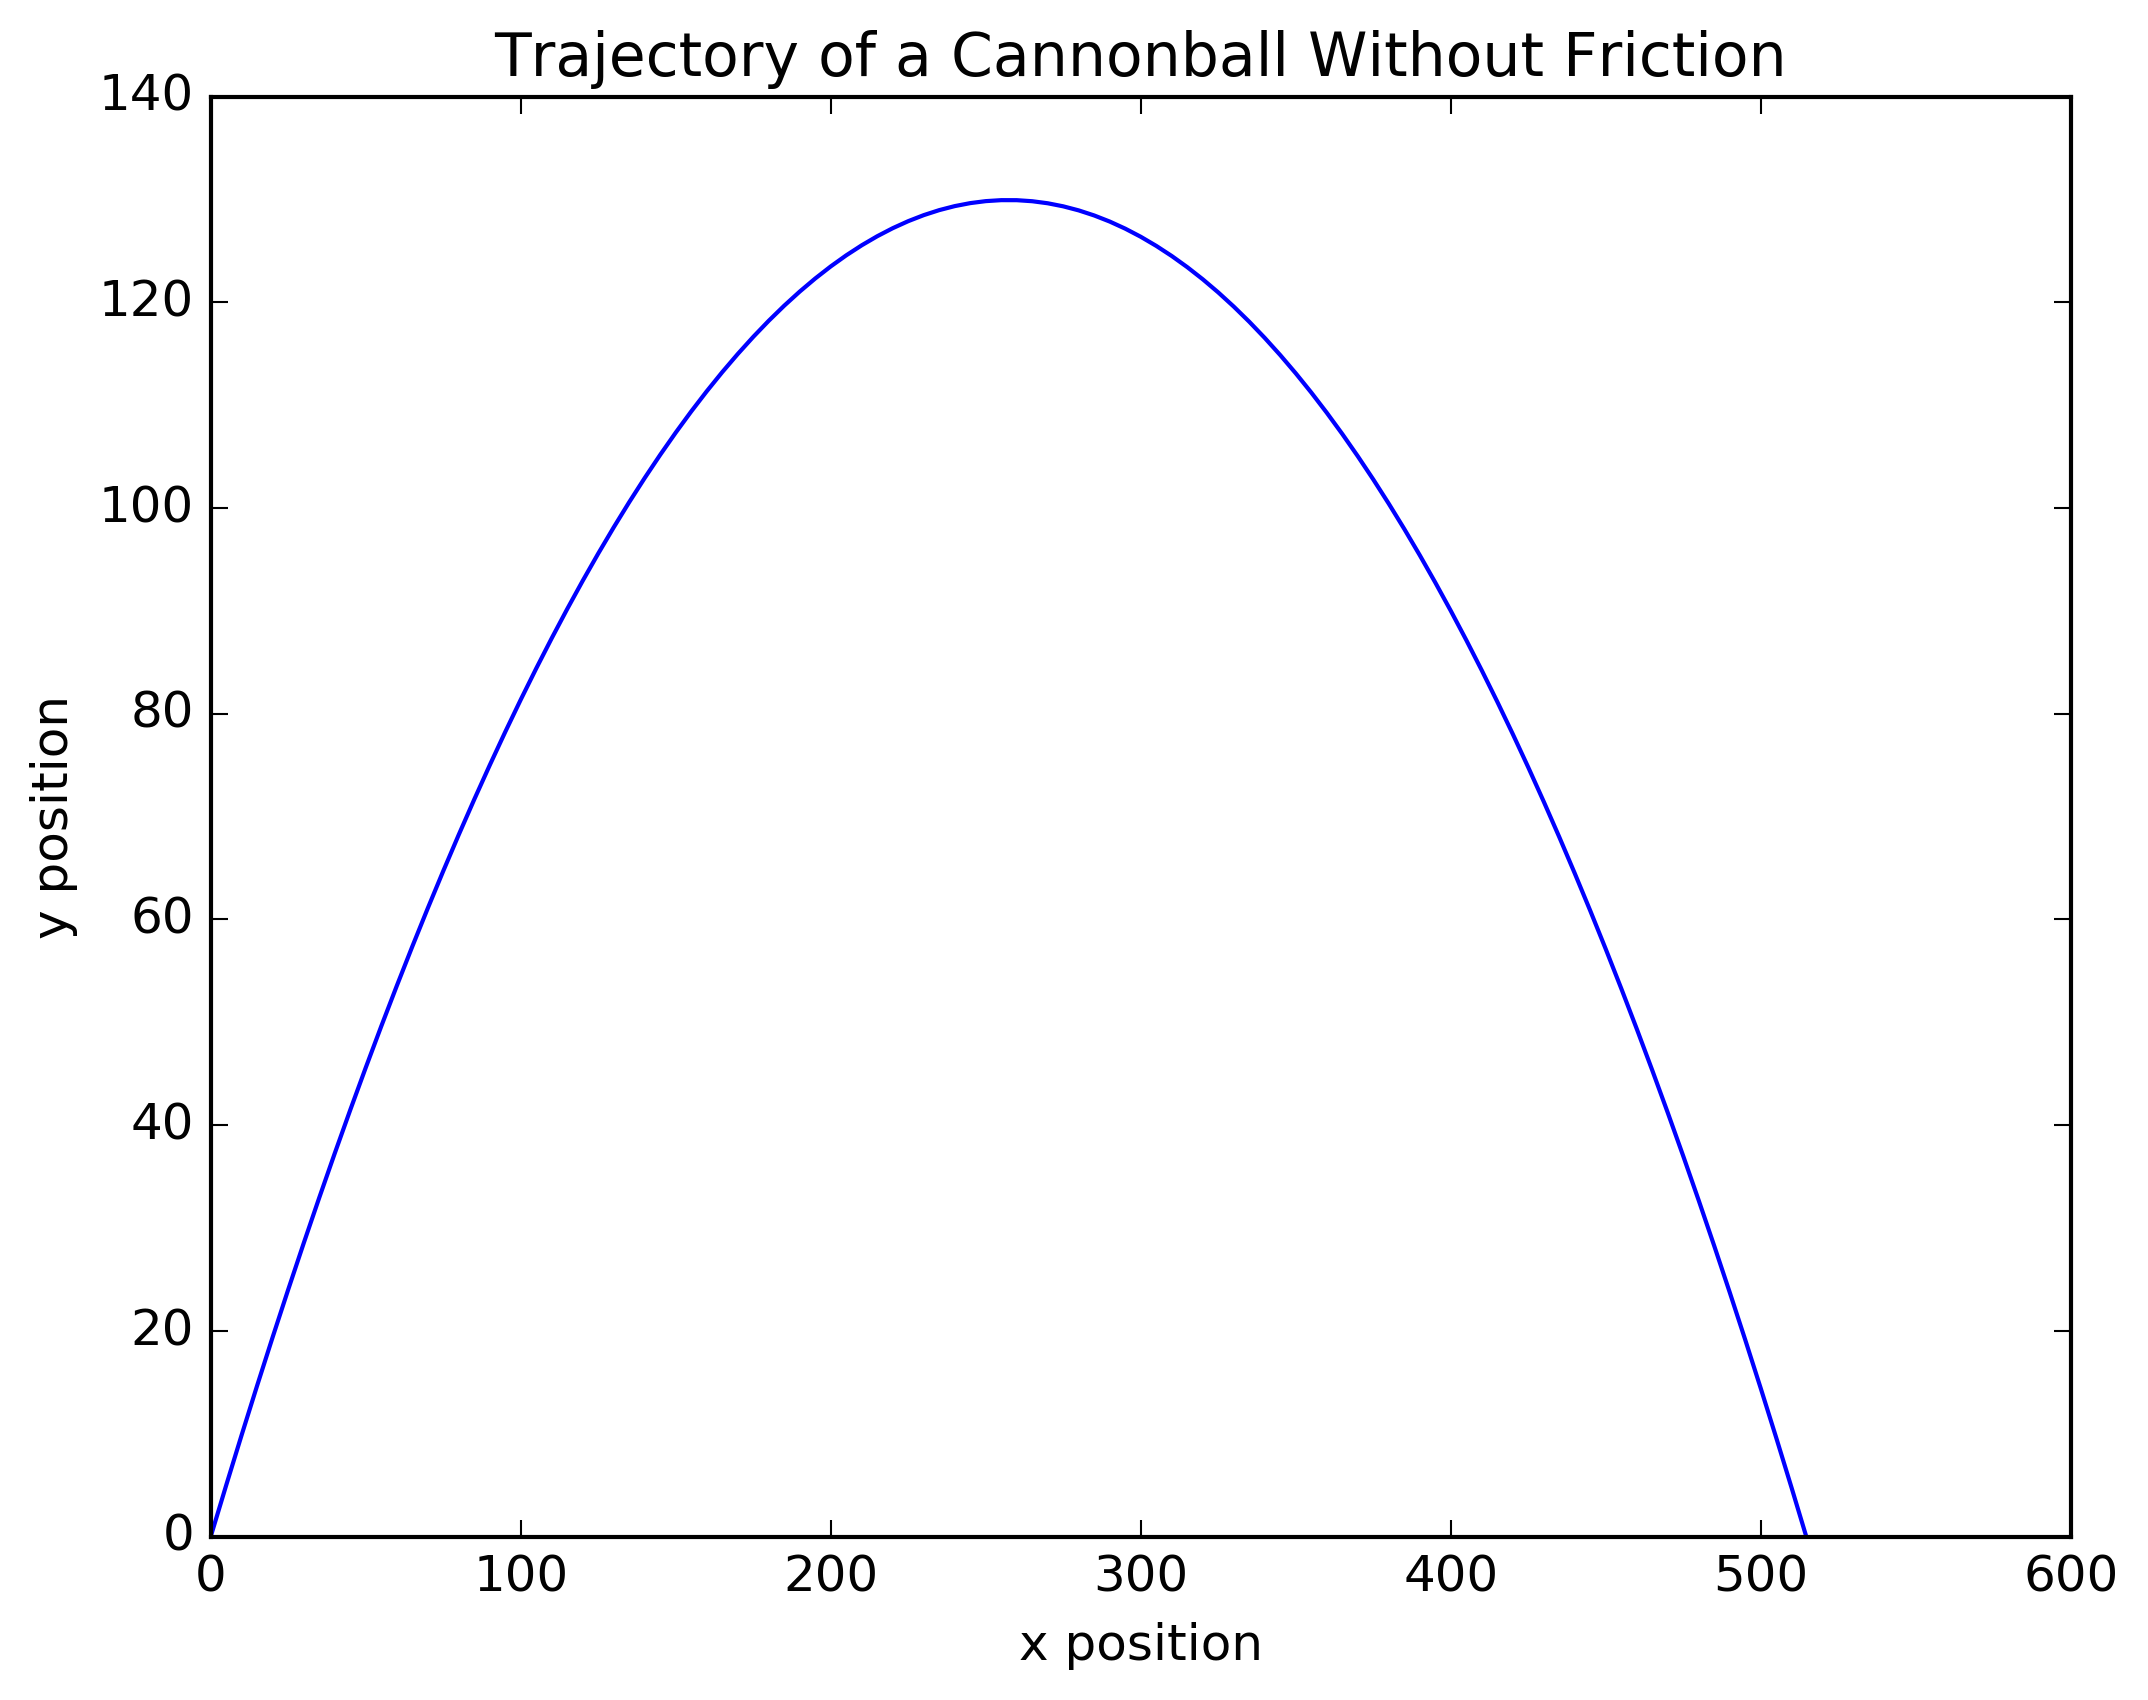
\includegraphics[width=0.7\linewidth]{../fig/cannonball1.png}
  \centering
  \caption{Trajectory of a cannonball with no friction using the simple Euler scheme}
  \label{fig:cannonball1}
\end{figure}

We integrate until the cannonball reaches the ground. The trajectory
can be seen in fig. \ref{fig:cannonball1}.




\end{document}
